\chapter{Statistical Data Analysis}

\section{Typical Analysis Procedure}

In "the old days" (before computers with almost unlimited computational power were available), the statistical analysis of data was typically restricted to hypothesis tests: you formulate a hypothesis, collect your data, and then accept or reject the hypothesis. The resulting hypothesis tests form the basic framework for by far most analyses in  medicine and life sciences, and the most important hypotheses tests will be described in the following chapters.

The advent of powerful computers has changed the game. Nowadays, the analysis of statistical data is (or at least should be) a highly interactive process: you look at the data, and generate models which may explain your data. Then you determine the best fit parameters for these models, and check these models, typically by looking at the residuals. If you are not happy with the results, you modify the model to improve the correspondence between models and data; when you are happy, you calculate the confidence interval for your model parameters, and form your interpretation based on these values. An introduction into this type of statistical analysis is provided in chapter \ref{chapter:Models}.

In either case, one should start off with the following steps:
\begin{itemize}
  \item Visually inspect the data.
  \item Find extreme samples, and check them carefully.
  \item Determine the data-type of the values.
  \item If the data are continuous, check whether or not they are normally distributed.
  \item Select and apply the appropriate test, or start with the model-based analysis of the data.
\end{itemize}

\subsection{Data Screening}

The first step in data analysis is the visual inspection of the data. Our visual system is enormously powerful, and if the data are properly displayed, trends that characterize the data can be clearly visible. In addition to checking if the first and the last data values have been read in correctly, it is recommendable to check for missing data and outliers.

\subsubsection{Outliers} \index{general}{outliers}

There is no unique definition for outliers. However, for normally distributed samples they are often defined as data that lie either more than 1.5*IQR (inter-quartile range), or more than 2 standard deviations, from the sample mean. Outliers often fall in one of two groups: they are either caused by mistakes in the recording, in which case they should be excluded; or they constitute very important and valuable data points, in which case they have to be included in the data analysis. To decide which of the two is the case, you have to check the underlying raw data (for saturation or invalid data values), and the protocols from your experiments (for mistakes that may have occurred during the recording). If an underlying problem is detected, then - and only then - one may eliminate the outliers from the analysis. In every other case, the data have to be kept!

\subsection{Normality Check} \index{general}{normality check}

Statistical hypothesis tests can be grouped into parametric tests\index{general}{parametric tests} and non-parametric tests\index{general}{non-parametric tests}. Parametric tests assume that the data can be well described by a distribution that is defined by one or more parameters, in most cases by a normal distribution. For the given data set, the best-fit parameters for this distribution are then determined, together with their confidence intervals, and interpreted.

However, this approach only works if the given data set is in fact well approximated by the chosen distribution. If not, the results of the parametric test can be completely wrong. In that case non-parametric tests have to be used which are less sensitive, but therefore do not depend on the data following a specific distribution.

\begin{figure}
  \centering
  \includegraphics[width=0.75\textwidth]{../Images/ProbPlot.png}\\
  \caption{Probability-Plot, to check for normality of distribution.}\label{fig:qqplot}
\end{figure}


\subsubsection{Probability-Plots}\index{general}{plots!probability plot} \index{general}{plots!probplot}

In statistics, different tools are available for the visual assessments of distributions. They are graphical methods for comparing two probability distributions by plotting their \glspl{quantile}, or closely related parameters, against each other:

\begin{description}
  \item[QQ-Plots] \index{general}{plots!qq-plot}The "Q" in \acrfull{qq-plot} stands for \emph{quantile}. The quantiles of a given data set are plotted against the quantiles of a reference distribution, typically the standard normal distribution.
  \item[PP-Plots] \index{general}{plots!pp-plot} Plot the CDF (cumulative-distribution-function) of a given data set against the CDF of a reference distribution.
  \item[Probability Plots] \index{general}{plots!probability plot} Plot the ordered values of a given data set against the quantiles of a reference distribution.
\end{description}

In all three cases the results are similar: if the two distributions being compared are similar, the points will approximately lie on the line $y = x$. If the distributions are linearly related, the points will approximately lie on a line, but not necessarily on the line $y = x$ (Figure \ref{fig:qqplotChi2}).

In \emph{Python}, the plot can be generated with the command

\begin{lstlisting}
    stats.probplot(data, plot=plt)
\end{lstlisting}

\begin{figure}
  \centering
  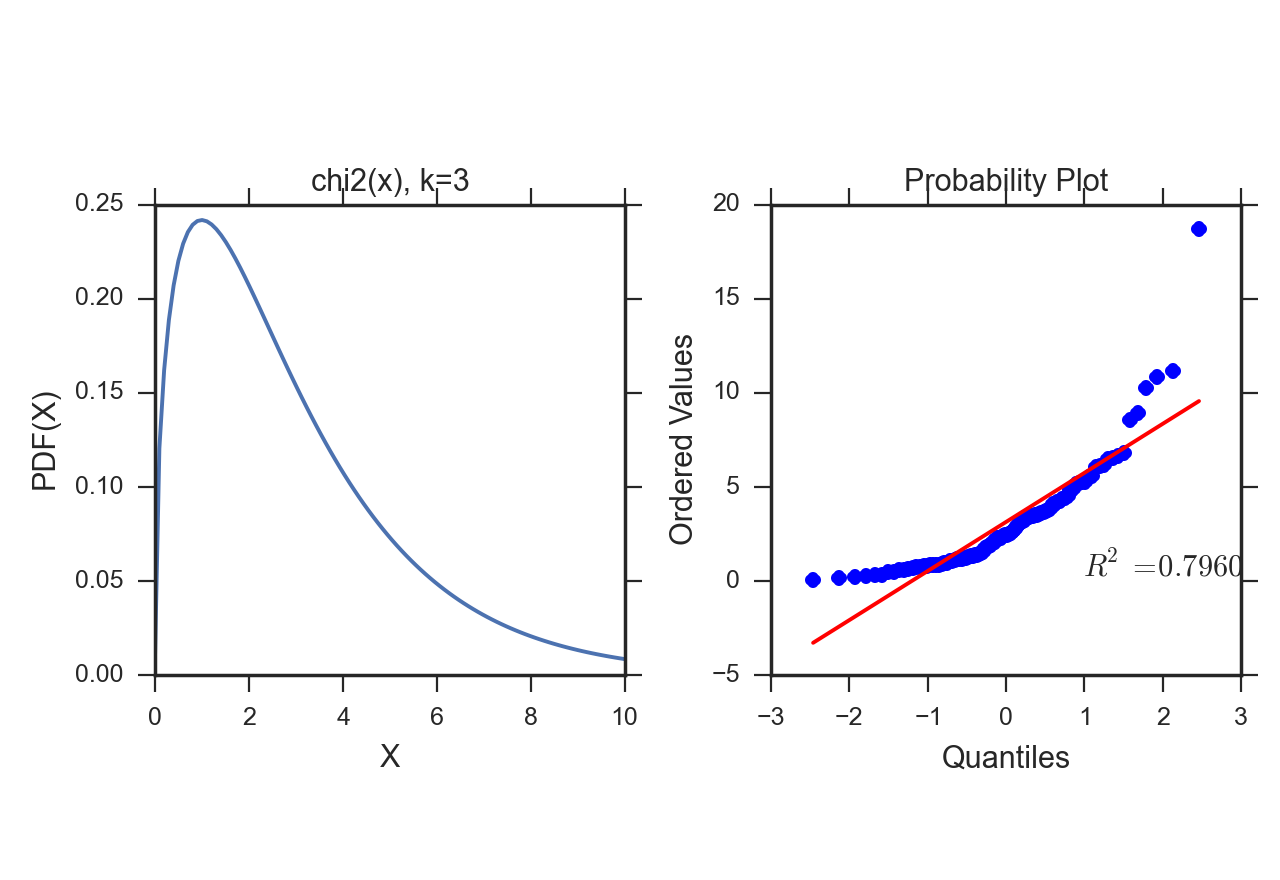
\includegraphics[width=1.0\textwidth]{../Images/chi2pp.png}\\
  \caption{Left) Probability-density-function for a Chi2-distribution (k=3), which is clearly non-normal. Right) Corresponding Probability-plot}\label{fig:qqplotChi2}
\end{figure}

To understand the principle behind those plots, look at the right plot in Fig. \ref{fig:qqplotChi2}. Here we have \emph{100} random datapoints from a chi2-distribution, which is clearly unsymmetrical. The x-value of the first data point is (approximately) the $1/100$-quantile of a standard normal distribution (\lstinline{stats.norm().ppf(0.01)}), which corresponds to \emph{-2.33} (The exact value is slightly shifted, because of a small correcton, called "Filliben's estimate"\index{general}{Filliben's estimate}). The y-value is the smallest value of our data-set. Similarly, the second x-value corresponds approximately to \lstinline{stats.norm().ppf(0.01)}, and the second y-value is the second-lowest value of the data set, etc.

\subsubsection{Hypothesis Tests for Normality}

In tests for normality, different challenges can arise: sometimes only few samples may be available, while other times one may have many data, but some extremely outlying values. To cope with the different situations different tests for normality have been developed. These tests to evaluate normality (or similarity to some specific distribution) can be broadly divided into two categories:

\begin{enumerate}
  \item Tests based on comparison (“best fit”) with a given distribution, often specified in terms of its CDF. Examples are the Kolmogorov-Smirnov test, the Lilliefors test, the Anderson-Darling test, the Cramér-von Mises criterion, as well as the Shapiro-Wilk and Shapiro-Francia tests.
  \item Tests based on descriptive statistics of the sample. Examples are the skewness test, the kurtosis test, the D’Agostino-Pearson omnibus test, or the Jarque-Bera test.
\end{enumerate}

For example, the Lilliefors test\index{general}{test!Lilliefors}, which is based on the Kolmogorov--Smirnov test \index{general}{test!Kolmogorov-Smirnov}, quantifies a distance between the empirical distribution function of the sample and the cumulative distribution function of the reference distribution, or between the empirical distribution functions of two samples. (The original Kolmogorov-Smirnov test should not be used if the number of samples is ca. $\leq 300$.)

The Shapiro-Wilk W test\index{general}{test!Shapiro-Wilk}, which depends on the covariance matrix between the order statistics of the observations, can also be used with $\leq 50$ samples, and has been recommended by \cite{altman99} and by \cite{Ghasemi2012c}.

The \emph{Python} command \lstinline{stats.normaltest(x)} uses the D’Agostino-Pearson \emph{omnibus test}\index{general}{test!omnibus}. This test combines a skewness and kurtosis test to produce a single, global, "omnibus" statistic.

\vspace{5 mm}

\PyImg "checkNormality.py" (p \pageref{py:checkNormality}) shows how to check graphically and quantitatively if a given distribution is normal.
\index{python}{checkNormality}

\begin{figure}
  \centering
  \includegraphics[width=0.5\textwidth]{../Images/KS_Example.png}\\
  \caption{Illustration of the Kolmogorov-Smirnov statistic. Red line is CDF, blue line is an ECDF, and the black arrow is the K-S statistic (from Wikipedia).}\label{fig:ksplot}
\end{figure}


\subsection{Transformation} \index{general}{transformation}
If your data deviate significantly from a normal distribution, it is sometimes possible to make the distribution approximately normal by transforming your data. For example, data often have values that can only be positive (e.g. the size of persons), and that have  long positive tail: such data can often be made normal by applying a log transform. This is demonstrated in Figure \ref{fig:lognormal}.


\section{Hypothesis tests}\label{sec:hypotheses} \index{general}{hypotheses}

\subsection{An Example}

Assume that you are running a private educational institution. Your contract says that if your students score 110 in the final exam, where the national average is 100, you get a bonus. When the results are significantly lower, you loose your bonus (because the students are not good enough), and you have to hire more teachers; and when the results are significantly higher, you also loose your bonus (because you have spent too much money on teachers), and you have to cut back on the number of teachers.

The final exam of your 10 students produce the following scores (Fig. \ref{fig:ExampleTtest}):

\begin{lstlisting}
  scores = array([ 109.4, 76.2, 128.7, 93.7, 85.6, 117.7, 117.2, 87.3, 100.3, 55.1])
\end{lstlisting}

\begin{figure}[ht]
  \centering
  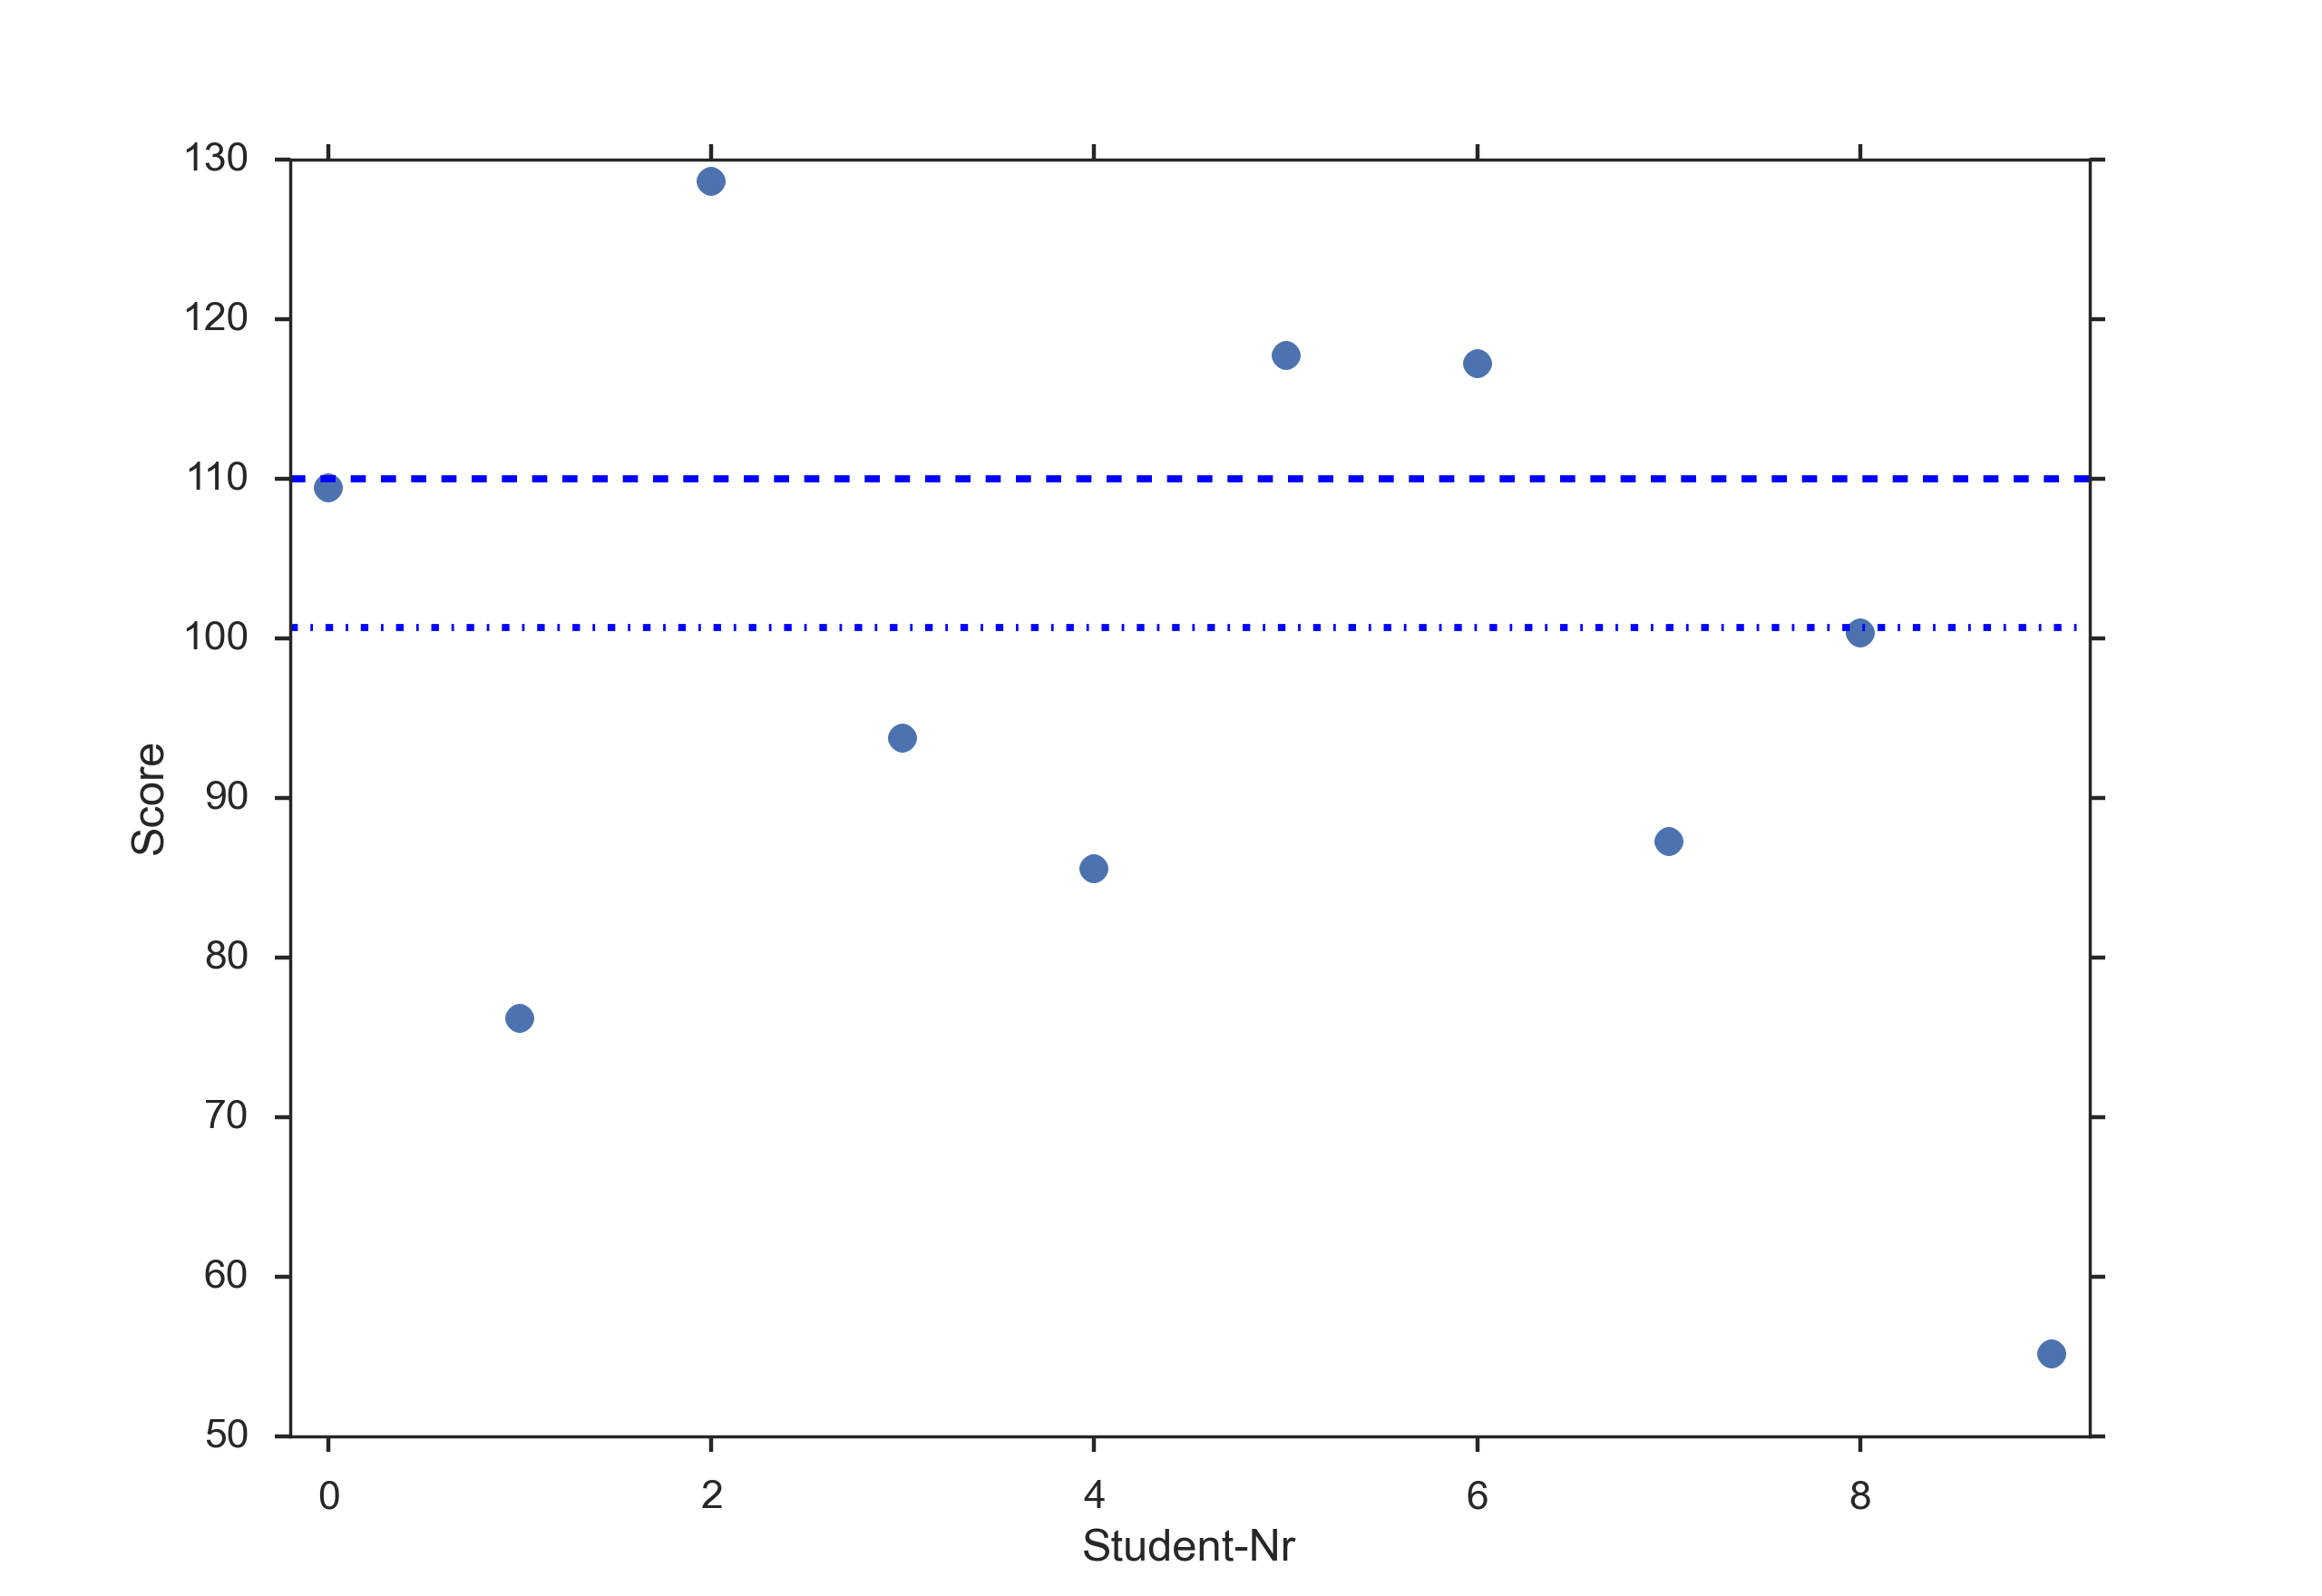
\includegraphics[width=0.75\textwidth]{../Images/fig_ExampleTtest.png}\\
  \caption{The question we ask: based on our sample mean (dashed-dotted line) and the observed variance of the data (the sample variance), do we believe that the population mean is different from 110 (dashed line)? Or in other words: our Null-hypothesis is that the difference between the population mean and 110 is zero. Can we keep our Null-hypothesis, or do we have to reject it based on the data?}\label{fig:ExampleTtest}
\end{figure}

The question we want to answer: Is the mean value of the scores (\emph{97.1}) significantly different from 110?

A \emph{normality test} (\lstinline{stats.normaltest(scores)}) indicates that the data are probably taken from a normal distribution.  Since we don't know the population variance of the results of students tested, we have to take our best guess, the sample variance (see also Fig. \ref{fig:population}). And we know that the normalized difference between sample and the population mean, the t-statistic, follows the t-distribution (Eq. \ref{eq:Tdistribution}).

The difference between our sample mean and the value we want to compare it to (\lstinline{ np.mean(scores) - 110} ) is \emph{12.9}. Normalized by the sample standard error (Eq. \ref{eq:Tdistribution}), this gives a value of \emph{t=-1.84}. Since the t-distribution is a known curve that depends only on the number of samples, and we can calculate the likelihood that we obtain a t-statistic of $|t| > 1.84$:

\begin{lstlisting}
    tval = (110-np.mean(scores))/stats.sem(scores)  # 1.84
    td = stats.t(len(scores)-1)                     # "frozen" t-distribution
    p = 2*td.sf(tval)                               # 0.0995
\end{lstlisting}

(The factor \emph{2} in the last line of the code is required, since we have to combine the probability of $t<-1.84$ and $t>1.84$.) Expressed in words, given our sample data, we can state that the likelihood that the population mean is \emph{110} is 9.95\%. But since a \emph{statistical difference} is only given by convention if the likelihood is less than 5\%, we conclude that the observed value of 97.1 is not significantly different from 110, and the bonus has to be paid out.

\subsection{Generalization}

Based on the previous example, the general procedure for hypothesis tests can be described as follows (the sketch in Fig. \ref{fig:population} indicates the meaning of many upcoming terms):

\begin{itemize}
  \item A random sample is drawn from a population. (In our example, the random sample is our \emph{scores}).
  \item A Null hypothesis\index{general}{null hypothesis} is formulated. ("There is Null difference between the population mean and the value of 110.")
  \item A test-statistic is calculated, from which we know the probability distribution. (Here the sample mean, since we know that the mean value of samples from a normal distribution follows the t-distribution.)
  \item Comparing the observed value of the statistic (here the obtained t-value) with the corresponding distribution (the t-distribution), we can find the likelihood that a value as extreme as or more extreme than s the observed one is found by chance. This is the so-called "p-value".
  \item If the p-value is $p<0.05$, we reject the Null-hypothesis, and speak of a "statistically significant difference". If a value of $p<0.001$ is obtained, the result is typically called "highly significant". The critical region of a hypothesis test is the set of all outcomes which cause the null hypothesis to be rejected in favor of the alternative hypothesis\index{general}{alternative hypothesis}.
\end{itemize}

In other words, the p-value states how likely it is to obtain a value as extreme or more extreme by chance alone, \emph{if the Null hypothesis is true}.

The value against which the p-value is compared is the "significance level"\index{general}{significance level}, and is often indicated with the letter $\alpha$. The significance level is a user choice, and typically set to $0.05$.

This way of proceeding to test a hypothesis is called Statistical Inference\index{general}{statistical inference}.

Remember, p only indicates the likelihood of obtaining a certain value for the test statistic if the null hypothesis is true - nothing else!

And keep in mind that improbable events do happen, even if not very frequently. For example, back in 1980 a woman named Maureen Wilcox bought tickets for both the Rhode Island lottery and the Massachusetts lottery. And she got the correct numbers for both lotteries. Unfortunately for her, she picked all the correct numbers for Massachusetts on her Rhode Island ticket, and all the  right numbers for Rhode island on her Massachusetts ticket :(  Seen statistically, the p-value for such an event would be extremely small - but it did happen anyway.

\subsubsection{Additional Examples}

\textbf{Example 1: } Let us compare the weight of two groups of subject. The Null hypothesis is that there is null difference in the weight between the two groups. If a statistical comparison of the weight produces a p-value of 0.03, this means that the probability that the null hypothesis is correct is 0.03, or 3\%. Since this probability is quite low, we say that "there is a significant difference between the weight of the two groups".

\textbf{Example 2: } If we want to check the assumption that the mean value of a group is 7, then the null hypothesis would be: "We assume that there is null difference between the mean value in our population and the value 7."

\subsection{The interpretation of the p-value, and the "p-value fallacy"}

\fbox{
\begin{minipage}{15 cm}
    \textbf{Note:} A value of $p<0.05$ for the null hypothesis has to be interpreted as follows: \emph{If the null hypothesis is true, the chance that we find a test statistic as extreme or more extreme than the one observed is less than 5\%.} This is \emph{not} the same as saying that the null hypothesis is false, and even less so, that an alternative hypothesis is true!
\end{minipage}
}

\vspace{5 mm}

Stating a p-value alone is no longer state-of-the-art for the statistical analysis of data. You should also state the confidence intervals for the parameter that you investigate.

Therefore research is sometimes divided into "exploratory research"\index{general}{exploratory research} and "confirmatory research"\index{general}{confirmatory research}. Take for example the case of Matt Motyl, a Psychology PhD student at the University of Virginia. In 2010, data from his study of nearly 2000 people indicated that political moderates saw shades of grey more accurately than people with more extreme political opinions, with a p-value of 0.01. However, when he tried to reproduce the data, the p-value dropped down to 0.59. So while the \emph{exploratory research} showed that a certain hypothesis may be likely, the \emph{confirmatory research} showed that the hypothesis did not hold (\cite{Nuzzo2014}).

\cite{sellke2001} have investigated this question in detail, and recommend to use a "calibrated p-value" to estimate the probability of making a mistake when rejecting the null hypothesis, when the data produce a p-value $p$:

\begin{equation}\label{eq:pFallacy}
    \alpha(p)= \frac{1}{1 + \frac{1}{-e \; p \; log(p)}}
\end{equation}

with $e=exp(1)$, and $log$ the natural logarithm. For example, $p=0.05$ leads to $\alpha=0.29$, and $p=0.01$ to $\alpha=0.11$.

\subsection{Types of Error}
In hypothesis testing, two types of errors can occur:

\subsubsection{Type I errors} \index{general}{error!Type I} \index{general}{power}
\gls{TypeI} are errors, where you get a significant result despite the fact that the hypothesis is true. The likelihood of a Type I error is commonly indicated with $\alpha$, and is set before you start the data analysis. In quality control, a Type I error is called Producer Risk, because you keep a produced item despite the fact that it meets the regulatory requirements.

For example, assume that the population of young Austrian adults has a mean IQ of 105 (i.e. we are smarter than the rest) and a standard deviation of 15. We now want to check if the average FH student in Linz has the same IQ as the average Austrian, and we select 20 students. We set $\alpha=0.05$, i.e. we set our significance level to 95\%.
Let us now assume that the average student has in fact the same IQ as the average Austrian. If we repeat our study 20 times, we will find one of those 20 times that our sample mean is significantly different from the Austrian average IQ. Such a finding would be a false result, despite the fact that our assumption is correct, and would constitute a type I error.

\subsubsection{Type II errors and Test Power}\index{general}{error!Type II}
If we want to answer the question "How much chance do we have to reject the null hypothesis when the alternative is in fact true?" Or in other words, "What’s the probability of detecting a real effect?" we are faced with a different problem. To answer these questions, we need an "alternative hypothesis".

For the example given above, an alternative hypothesis could be: "We assume that our population has a mean value of 6."

A \gls{TypeII} is an error, where you do \emph{not} get a significant result, despite the fact that the null-hypothesis is false.  In quality control, a Type II error is called a Consumer Risk, because the consumer obtains an item that does not meet the regulatory requirements.

The probability for this type of error is commonly indicated with $\beta$. The "power" of a statistical test is defined as $(1-\beta)*100$, and is the chance of correctly accepting the alternate hypothesis. Figure \ref{fig:power1} shows the meaning of the power of a statistical test. Note that for finding the power of a test, you need an alternative hypothesis.

\subsubsection{Type II Errors and P-value}

In other words, p values are often used to measure evidence against a hypothesis. Unfortunately, they are often incorrectly viewed as an error probability for rejection of the hypothesis, or, even worse, as the posterior probability (i.e. after the data have been collected) that the hypothesis is true. As an example, take the case where the alternative hypothesis is that the mean is just a fraction of one standard deviation larger than the mean under the null hypothesis: in that case, a sample that produces a p-value of 0.05 may just as likely be produced if the alternative hypothesis is true as if the null hypothesis is true!

\subsection{Sample Size}\index{general}{sample size}
The power of a statistical test depends on four factors:

\begin{enumerate}
  \item  $\alpha$, the probability for Type I errors
  \item  $\beta$, the probability for Type II errors ( $\Rightarrow$ power of the test)
  \item  $d$, the effect size, i.e. the magnitude of the investigated effect relative to $\sigma$, the standard deviation of the sample
  \item  $n$, the sample size
\end{enumerate}

Only 3 of these 4 parameters can be chosen, the $4^{th}$ is then automatically fixed.

The absolute size of the difference $D$ between mean treatment outcomes that will answer the clinical question being posed is often called Clinical Significance or Clinical Relevance.

\begin{figure}[!ht]
  \centering
  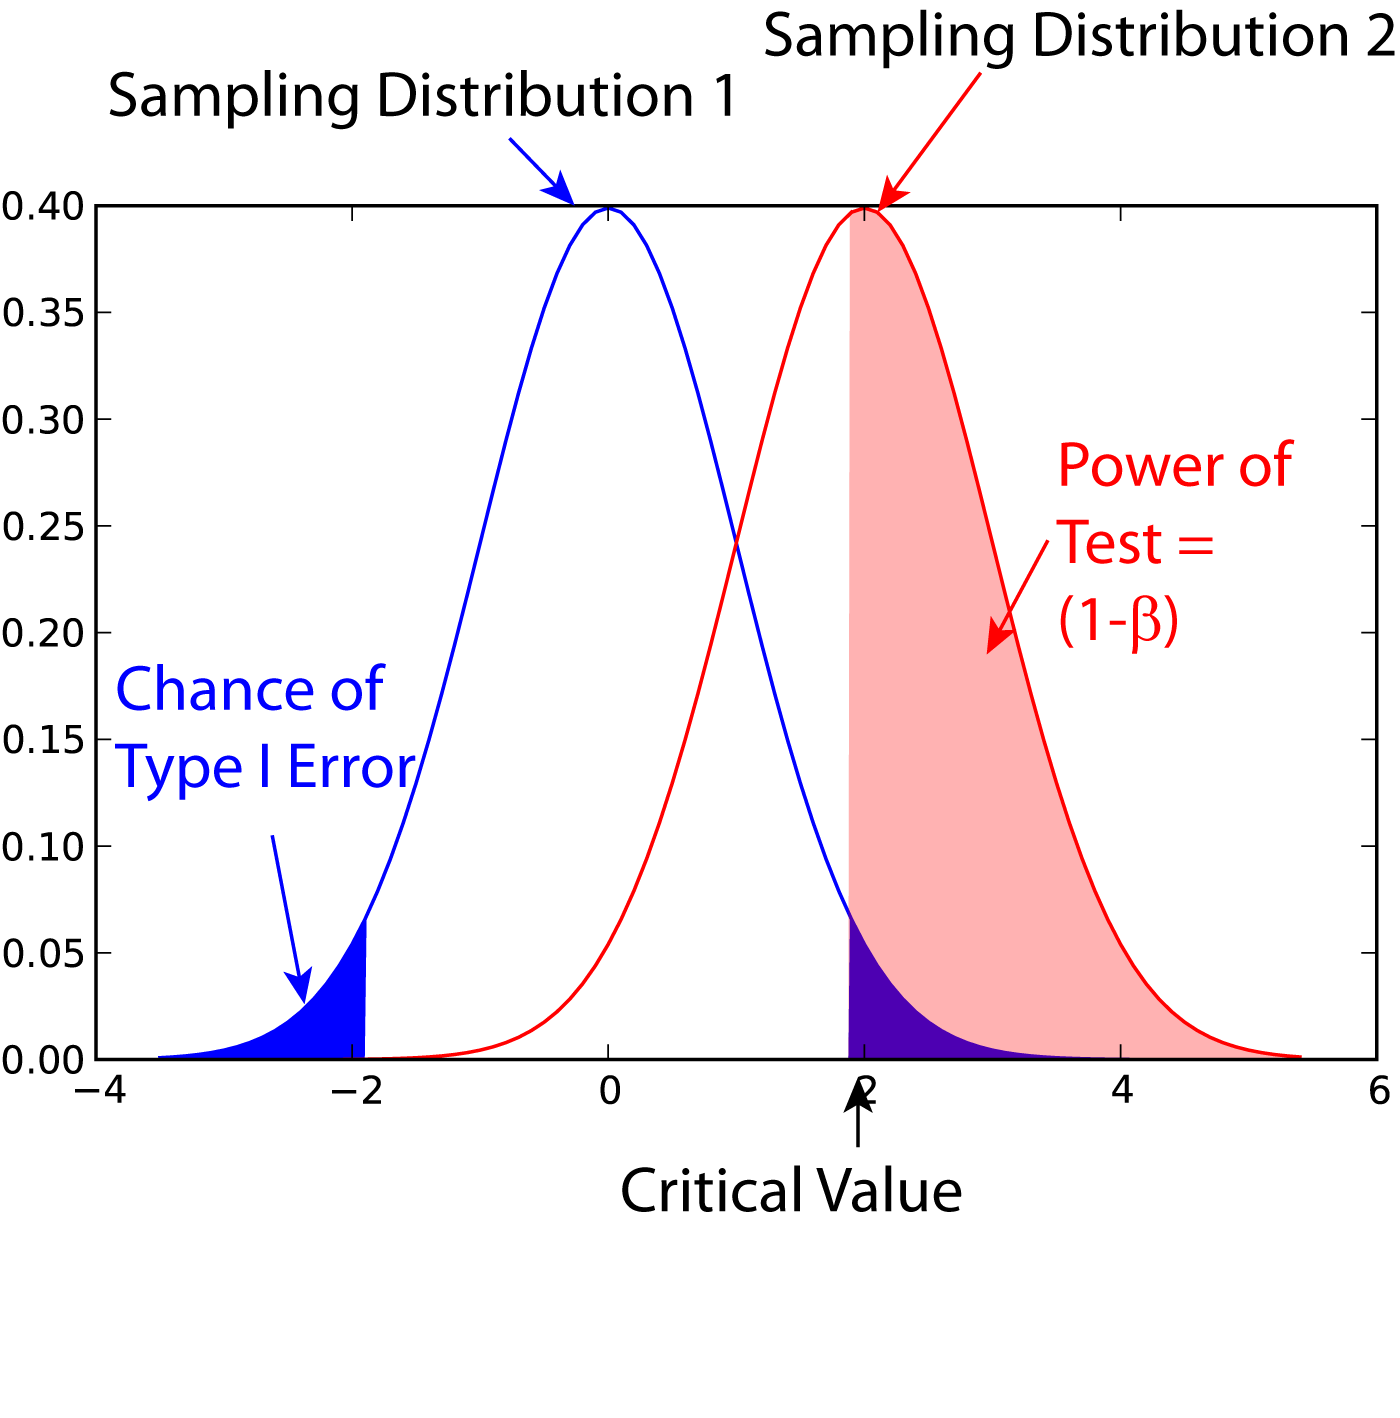
\includegraphics[width=0.5\textwidth]{../Images/power1.png}\\
  \caption{\emph{Power} of a statistical test, for comparing the mean value of two sampling distributions.}\label{fig:power1}
\end{figure}

\begin{figure}[!ht]
  \centering
  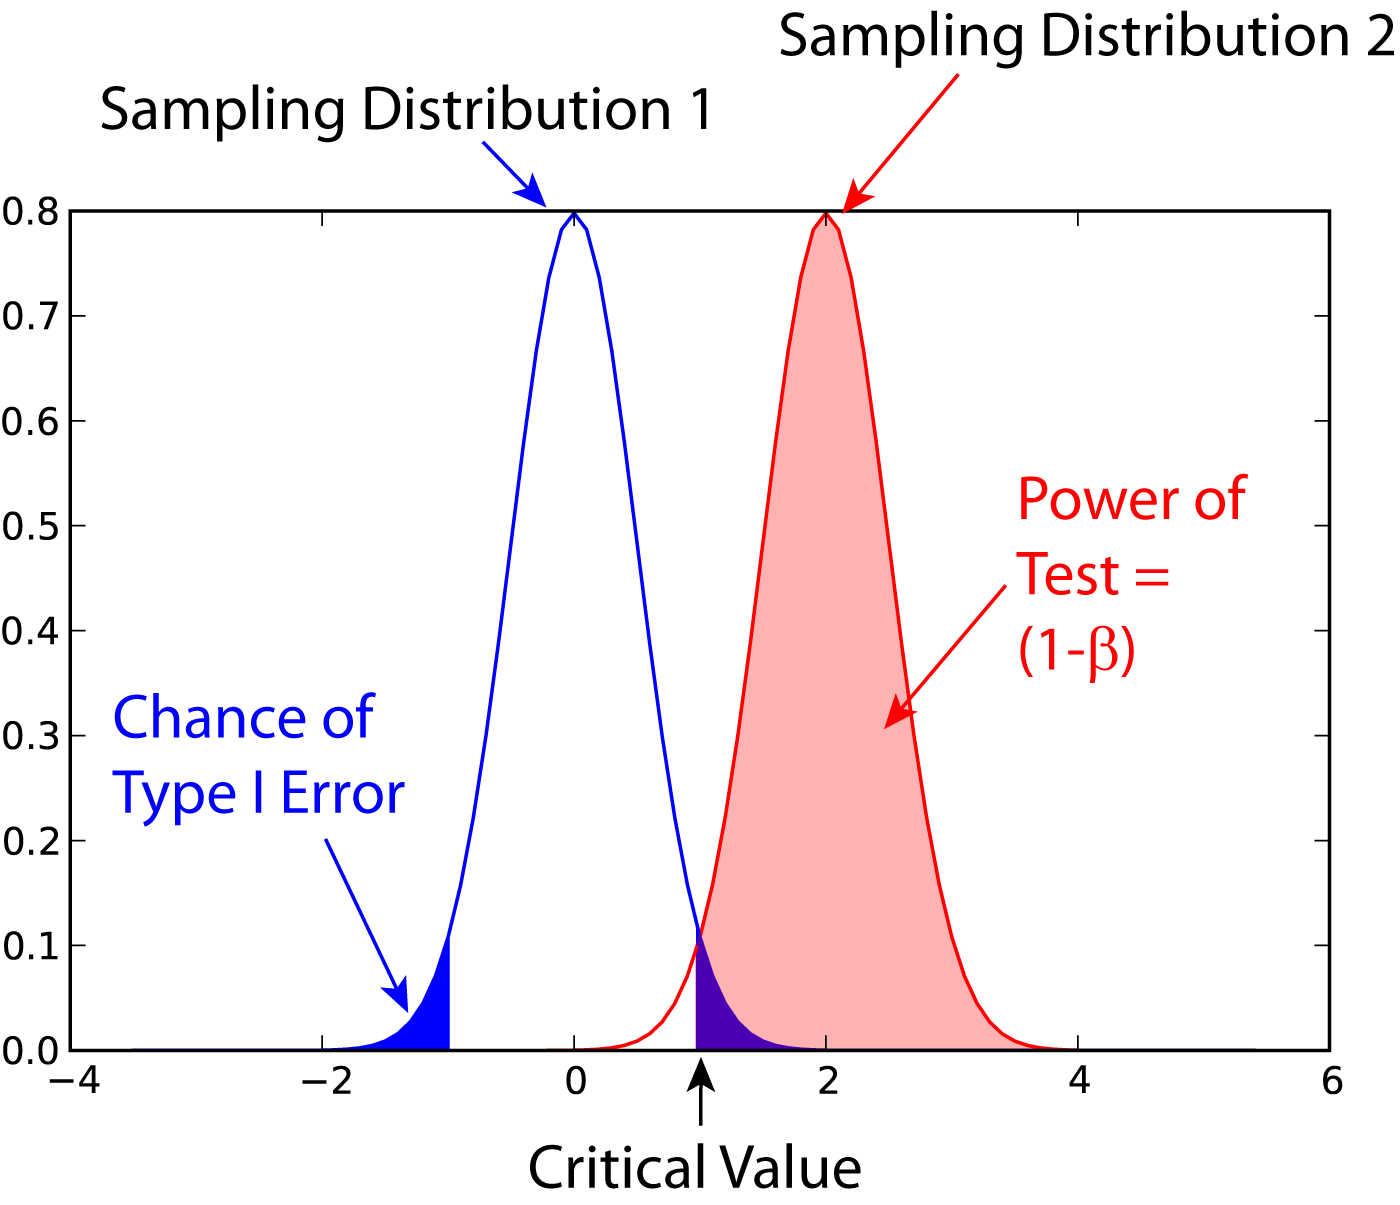
\includegraphics[width=0.5\textwidth]{../Images/power2.png}\\
  \caption{Effect of an increase in sampling size on the power of a test.}\label{fig:power2}
\end{figure}

\subsubsection{Examples for some special cases}

\paragraph{Test on One Mean}
If we have the hypothesis that the data population has a mean value of $x_1$ and a standard deviation of $\sigma$, and the actual population has a mean value of $x_1+D$ and the same standard deviation, we can find such a difference with a minimum sample number of

\begin{equation}
  n = \frac{{({z_{1 - \alpha /2}} + {z_{1 - \beta }})}^2}{d^2}
\end{equation}

Here $z$ is the standardized normal variable (see also chapter \ref{sec:normalDistribution})

\begin{equation}
  z = \frac{x-\mu}{\sigma} .
\end{equation}

and $d = \frac{D}{\sigma}$ the effect size.

In words, if the real mean has a value of $x_1$, we want to detect this correctly in at least $1-\alpha\%$ of all tests; and if the real mean is shifted by $D$ or more, we want to detect this with a likelihood of at least $1-\beta\%$.

\paragraph{Test Between Two Different Populations}
For finding a difference between two normally distributed means, with standard deviations of $\sigma_1$ and $\sigma_2$, the minimum number of samples we need in each group to detect an absolute difference $D$ is

\begin{equation}
  {n_1} = {n_2} = \frac{{({z_{1 - \alpha /2}} + {z_{1 - \beta }})}^2(\sigma _1^2 + \sigma _2^2)}{D^2} .
\end{equation}

\subsubsection{Python Solution}

\emph{statsmodels} makes clever use of the fact that 3 of the 4 factors mentioned above are independent, and combines it with the \emph{Python} feature of "named parameters" to provide a program that takes 3 of those parameters as input, and calculates the remaining $4^{th}$ parameter. For example,

\begin{lstlisting}
    In [1]: from statsmodels.stats import power

    In [2]: nobs = power.tt_ind_solve_power(effect_size = 0.5, alpha =0.05, power=0.8)
    In [3]: print(nobs)
    Out[3]: 63.76561177540974
\end{lstlisting}

tells us that if we compare two groups with the same number of subjects and the same standard deviation, require an $\alpha=0.05$ a test power of $80\%$, and we want to detect a difference between the groups that is half the standard deviation, we need to test 64 subjects.

Similarly,

\begin{lstlisting}
    In [4]: effect_size = power.tt_ind_solve_power(alpha =0.05, power=0.8, nobs1=25)
    In [5]: print(effect_size)
    Out[5]: 0.8087077886680407
\end{lstlisting}

tells us that if we have an $\alpha=0.05$, a test power of $80\%$, and 25 subjects in each group, then the smallest difference between the groups is 81\% of the sample standard deviation.

The corresponding command for one sample t-tests is \lstinline{tt_solve_power}.

\subsubsection{Programs: SampleSize}

\PyImg "sampleSize.py" (p \pageref{py:sampleSize}): sample size calculation for normally distributed groups with arbitrary standard deviations.
\index{python}{sampleSize}


\section{Sensitivity and Specificity}

Some of the more confusing terms in statistical analysis are \gls{sensitivity} \index{general}{sensitivity} and \gls{specificity} \index{general}{specificity}. A related topic are the "positive predictive value (PPV)" \index{general}{positive predictive value} and the "negative predictive value (NPV)" \index{general}{negative predictive value}. The following diagram shows how the four are related:

\begin{figure}[ht]
  \centering
  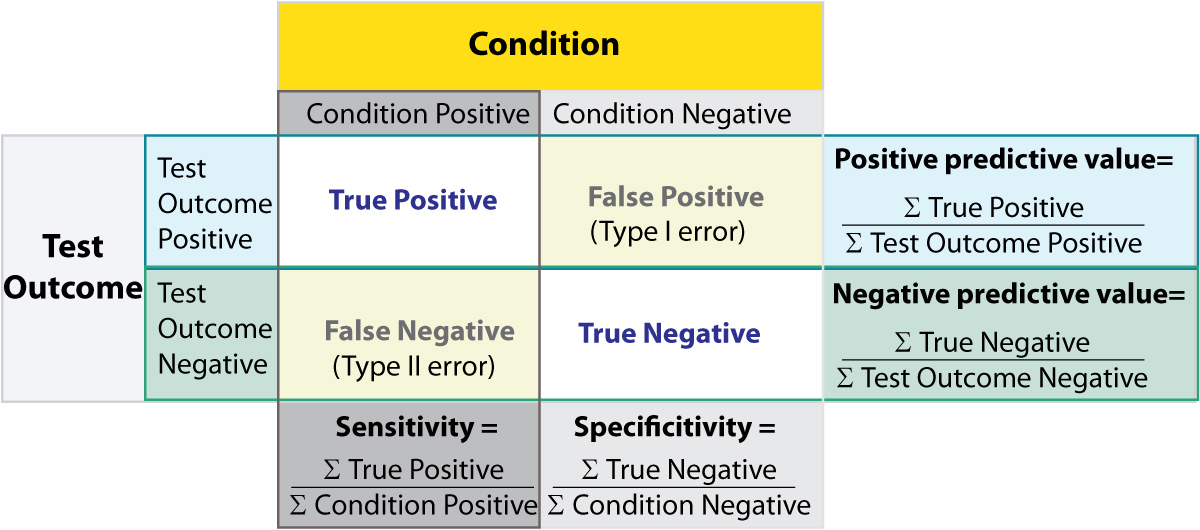
\includegraphics[width=0.9\textwidth]{../Images/Sensitivity_Specificity_Diagram.jpg}\\
  \caption{Relationship between sensitivity, specificity, positive predictive value and negative predictive value.}\label{fig:sens_spec_diagram}
\end{figure}

\begin{description}
  \item[Sensitivity] Also called \gls{power}. Proportion of positives that are correctly identified by a test = probability of a positive test, given the patient is ill.
  \item[Specificity] Proportion of negatives that are correctly identified by a test = probability of a negative test, given that patient is well.
  \item[Positive Predictive Value (PPV)] Proportion of patients with positive test results who are correctly diagnosed.
  \item[Negative Predictive Value (NPV)] Proportion of patients with negative test results who are correctly diagnosed.
\end{description}

For example, pregnancy tests have a high sensitivity: when a woman is pregnant, the probability that the test is positive is very high.

In contrast, an indicator for an attack with atomic weapons on the White House should have a very high specificity: if there is no attack, the probability that the test goes on should be very, very small.

Sensitivity and specificity characterize a test, while PPV and NPV are the parameters that tell the doctor how to interpret a test result.

While sensitivity and specificity characterise a test and are independent of prevalence, they do not indicate what portion of patients with abnormal test results are truly abnormal. This information is provided by the positive/negative predictive value. However, as Fig. \ref{fig:prevalence} indicates, these values are affected by the prevalence \index{general}{prevalence} of the disease. The "prevalence" of a disease indicates how many out of 100'000 people are affected by it; in contrast, the "incidence" gives the number of newly diagnosed cases per 100'000 people. In summary, we need to know the prevalence of the disease as well as the PPV/NPV of a test to provide a sensible interpretation of the test results.

\begin{figure}[ht]
  \centering
  \includegraphics[width=0.75\textwidth]{../Images/Sensitivity_Specificity.png}\\
  \caption{Effect of prevalence on PPV and NPV. "T" stands for "test", and "P" for "patient". (For comparison with below: T+P+ = TP, T-P- = TN, T+P- = FP, and T-P+ = FN)} \label{fig:prevalence}
\end{figure}

Figure \ref{fig:sens_spec_example} gives a worked example:

\begin{figure}[ht]
  \centering
  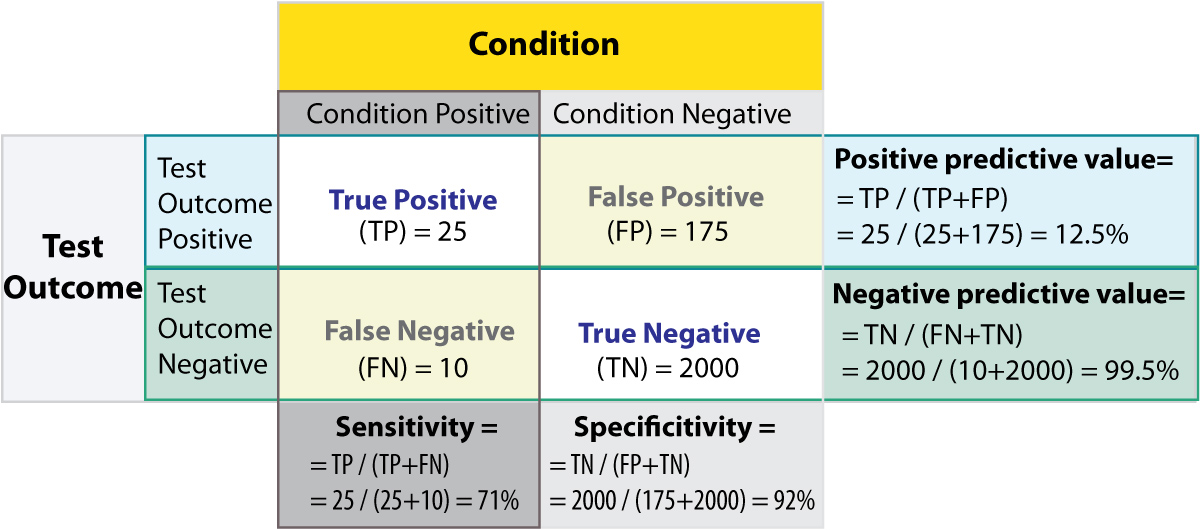
\includegraphics[width=0.9\textwidth]{../Images/Sensitivity_Specificity_Example.jpg}\\
  \caption{Worked example.}\label{fig:sens_spec_example}
\end{figure}

\paragraph{Related calculations}

\begin{itemize}
  \item False positive rate ($\alpha$) = type I error = $1 - specificity$ = $\frac{FP}{FP + TN}$ = $\frac{180}{180+1820}$ = 9\%
  \item False negative rate ($\beta$) = type II error = $1 - sensitivity$ = $\frac{FN}{TP + FN}$ = $\frac{10}{20+10}$ = 33\%
  \item Power = sensitivity = $1 - \beta$
  \item Likelihood ratio positive = $\frac{sensitivity}{1−specificity}$ = $\frac{66.67\%}{1−91\%}$ = 7.4
  \item Likelihood ratio negative = $\frac{1−sensitivity}{specificity}$ = $\frac{1−66.67\%}{91\%}$ = 0.37
\end{itemize}

Hence with large numbers of false positives and few false negatives, a positive test outcome in this example is in itself poor at confirming cancer (PPV = 12.5\%) and further investigations must be undertaken; it did, however, correctly identify 71\% of all cancers (the sensitivity). However as a screening test, a negative result is very good at reassuring that a patient does not have cancer (NPV = 99.5\%) and at this initial screen correctly identifies 92\% of those who do not have cancer (the specificity).

\section{ROC Curve}\index{general}{ROC curve}

Closely related to sensitivity and specificity is the \acrfull{roc} (ROC) curve. This is a graph displaying the relationship between the true positive rate (on the vertical axis) and the false positive rate (on the horizontal axis). The technique comes from the field of engineering, where it was developed to find the predictor which best discriminates between two given distributions. In the ROC-curve (Figure \ref{fig:ROC}) this point is given by the value with the largest distance to the diagonal.

\begin{figure}[ht]
  \centering
  \includegraphics[width=0.75\textwidth]{../Images/ROC.png}\\
  \caption{Top: Probability density functions for two distributions. Bottom: corresponding \emph{ROC-curve}.}\label{fig:ROC}
\end{figure}

\section{Common Statistical Tests for Comparing Groups}

Table \ref{table:tests} gives an overview of the most common statistical tests for different combinations of data.
\begin{table}
  \centering
  \footnotesize{
  \begin{tabular}{ | p{5cm} || p{5cm} | p{5cm} | }
     \hline
     No. of Groups Compared  & \textbf{Independent Samples} & \textbf{Paired Samples} \\ \hline
     \textbf{Groups of Nominal Data} & & \\ \hline
     2 or more & Fisher's exact test or Chi-Square test & McNemar's test \\ \hline
     \textbf{Groups of Ordinal Data} & & \\ \hline
     2 & Mann-Whitney U test & Wilcoxon signed rank test \\ \hline
     3 or more & Kruskal-Wallis test & Friedman test \\ \hline
     \textbf{Groups of Continuous Data} & & \\ \hline
     2 & Student's t-test or Mann-Whitney test & Paired t-test or Wilcoxon signed-rank test \\ \hline
     3 or more & ANOVA or Kruskal-Wallis test & Repeated Measures ANOVA or Friedman test \\ \hline

  \end{tabular}
  }

  \caption{Typical tests for statistical problems.}\label{table:tests}
\end{table}

\subsection{Examples}

\begin{description}
  \item[2 groups, nominal] male/female, blond-hair/black-hair. E.g. "Are females more blond than males?"
  \item[2 groups, nominal, paired] 2 labs, analysis of blood samples. E.g. "Does the blood analysis from Lab1 indicate more infections than the analysis from Lab2?"
  \item[2 groups, ordinal] black/white, ranking 100m sprint. E.g. "Are black sprinters more successful than white sprinters?"
  \item[2 groups, ordinal, paired] sprinters, before/after diet. E.g. "Does a chocolate diet make sprinters more successful?"
  \item[3 groups, ordinal] black/white/chinese, ranking 100m sprint. E.g. "Does ethnicity have an effect on the success of sprinters?"
  \item[3 groups, ordinal, paired] sprinters, before/after diet. E.g. "Does a rice diet make Chinese sprinters more successful?"
  \item[2 groups, continuous] male/female, IQ. E.g. "Are women more intelligent than men?"
  \item[2 groups, continuous, paired] male/female, looking at diamonds. E.g. "Does looking at diamonds raise the female heart-beat more than the male?
  \item[3 groups, continuous] Tyrolians, Viennese, Styrians; IQ. E.g. "Are Tyrolians smarter than people from other Austrian federal states?"
  \item[3 groups, continuous, paired] Tyrolians, Viennese, Styrians; looking at mountains. E.g. "Does looking at mountains raise the heartbeat of Tyrolians more than those of other people?"
\end{description}

\section{Exercises}
\begin{enumerate}
  \item
  \begin{enumerate}
    \item Read in the data from 'Data\textbackslash amstat\textbackslash calcium.dat.txt'.
    \item Check for erroneous entries.
    \item Check the Alkaline Phosphatase levels for normality. Use a log-transform on the data, and re-check.
  \end{enumerate}

\end{enumerate}

